\subsection{Page conditioning and line segmentation}
\label{sec:segmentation}

This subsection turns a photograph of a handwritten page into clean, deskewed, white-background line images for the text recogniser of Section~\ref{sec:textrec} and the writer classifier of Section~\ref{sec:writerid} (functional units FU~2.1 and FU~2.2; requirement R2), component by component: the array primitives the rest of the block is built from, lighting and binarisation, deskew, removal of what is not handwriting, line pitch and centres, and finally the seam cut and crop.

The deployed implementation is \texttt{SegmentLean.py}, eleven functions in about 570 lines behind a single entry point, \texttt{SegmentLines(path)}. The web server, the style-profile builder and the writer-classifier trainer all call that same entry point, so training pages are cut by exactly the code that cuts a page during normal use. Published methods are cited where they are used, and the rules around them are plain array arithmetic written for this project. No part of this block resamples through an imaging library: every operation that changes a pixel value is performed by the project's own module, implementing Equation~\ref{eq:seg-resize} directly; the library is used only to read the file from disk and to write the optional debug overlay.

\subsubsection{Design goals and the measured scale unit}

A flat-bed scan can be conditioned by grey conversion, binarisation and bounding-box line separation, which is what published pipelines do~\cite{hemanth2022,chen2023}. A photograph is harder: it adds uneven illumination, the surroundings of the sheet, skew, printed rules, edge slivers, creases, and lines that touch each other. The block therefore has three design goals: it must work at any camera resolution and any handwriting size without manual tuning, it must never delete handwriting to remove a nuisance, and it must keep as few fixed constants as possible. All three are met by letting the page set its own scale: the photograph is reduced $2{:}1$ per axis by box averaging, and the \emph{line pitch} $P$ is measured on that working image (Section~\ref{sec:seg-pitchcentres}), after which almost every threshold is a multiple of $P$ rather than an absolute pixel count. Only four constants are absolute: the blur radius, the floor of 60 ink pixels per emitted line, the $64\times640$ canvas size and the dynamic-programme weights (Table~\ref{tab:seg-const}, Appendix~\ref{sec:app-seg}).

Before any of the thresholds above can be fixed, the line itself needs a shared vocabulary. Every subsystem from here onwards measures handwriting against five quantities shown in Figure~\ref{fig:seg-geom}: the \emph{baseline}, the \emph{x-height} $x_{\mathrm h}$ (the height of a lower-case letter with no tall part and no tail), an \emph{ascender} and \emph{descender} reaching above and below that, and the \emph{line pitch} $P$, the baseline-to-baseline distance. The pitch $P$ is the unit of this block, because segmentation separates one line from the next; the x-height $x_{\mathrm h}$ is the unit of everything downstream (Sections~\ref{sec:wid-strokenorm}, \ref{sec:styleprofile}, \ref{sec:synthesis}), because measuring in x-heights removes both the camera's distance and the writer's absolute size as variables, so one stored style profile can be drawn at any pen size.

\begin{figure}[h]
\centering
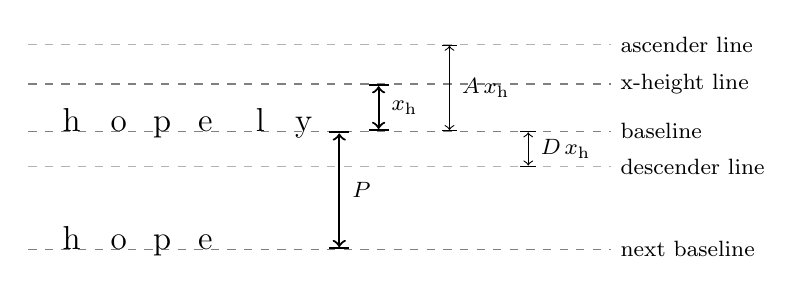
\begin{tikzpicture}[x=1cm,y=1cm,font=\footnotesize]
\draw[dashed,gray]      (0,0)    -- (7.4,0)    node[right,black]{baseline};
\draw[dashed,gray]      (0,0.6)  -- (7.4,0.6)  node[right,black]{x-height line};
\draw[dashed,gray!60]   (0,1.1)  -- (7.4,1.1)  node[right,black]{ascender line};
\draw[dashed,gray!60]   (0,-0.45)-- (7.4,-0.45)node[right,black]{descender line};
\node[anchor=base,font=\large] at (0.55,0) {h};
\node[anchor=base,font=\large] at (1.15,0) {o};
\node[anchor=base,font=\large] at (1.70,0) {p};
\node[anchor=base,font=\large] at (2.25,0) {e};
\node[anchor=base,font=\large] at (2.95,0) {l};
\node[anchor=base,font=\large] at (3.50,0) {y};
\draw[|<->|,thick] (4.45,0) -- (4.45,0.6) node[midway,right=1pt]{$x_{\mathrm{h}}$};
\draw[|<->|] (5.35,0) -- (5.35,1.1)  node[midway,right=1pt]{$A\,x_{\mathrm{h}}$};
\draw[|<->|] (6.35,0) -- (6.35,-0.45)node[midway,right=1pt]{$D\,x_{\mathrm{h}}$};
\draw[dashed,gray] (0,-1.5) -- (7.4,-1.5) node[right,black]{next baseline};
\node[anchor=base,font=\large] at (0.55,-1.5) {h};
\node[anchor=base,font=\large] at (1.15,-1.5) {o};
\node[anchor=base,font=\large] at (1.70,-1.5) {p};
\node[anchor=base,font=\large] at (2.25,-1.5) {e};
\draw[|<->|,thick] (3.95,0) -- (3.95,-1.5) node[midway,right=1pt]{$P$};
\end{tikzpicture}
\caption{The five quantities every subsystem measures handwriting against. $A>1$ because an ascender reaches above the x-height line, and $D<0$ because a descender falls below the baseline. $P$ is the unit used by this block; $x_{\mathrm h}$ is the unit used by every block after it.}
\label{fig:seg-geom}
\end{figure}

\subsubsection{Array primitives: summed-area tables and run tests}

Almost every operation in this block is a sum, a maximum, or a test of whether anything is set, taken over a rectangular window. Computed directly, a window of radius $r$ costs $O(r)$ per pixel per axis, too slow here because the illumination blur below uses a radius of up to 40 pixels. The module therefore builds a summed-area table~\cite{crow1984}, also called an integral image, in one $O(HW)$ pass of two cumulative sums, after which the sum over a window of \emph{any} size costs four look-ups instead of $(2r+1)^2$ additions. Three stages of this block resample an image, and each does so by bilinear interpolation at the source position given by Equation~\ref{eq:seg-resize}, the one exception being an ownership map resampled by nearest neighbour, because its values are integer line indices that interpolation would invent new values for:
\begin{equation}
y_s=\frac{(i+0.5)\,h}{h'}-0.5,\quad x_s=\frac{(j+0.5)\,w}{w'}-0.5,\quad I'(i,j)=\sum_{a,b\in\{0,1\}}\omega_{ab}\,I(\lfloor y_s\rfloor+a,\lfloor x_s\rfloor+b).
\label{eq:seg-resize}
\end{equation}

The table itself is the running two-dimensional sum of the image,
\begin{equation}
S(y,x)=\sum_{i<y}\sum_{j<x} I(i,j),
\label{eq:seg-sat}
\end{equation}
where $S$ is the summed-area table and $I$ the image being summed. Equation~\ref{eq:seg-sat} is built once per image. Any window sum is then read from four of its entries,
\begin{equation}
\mathrm{BoxSum}=S(y_2,x_2)-S(y_1,x_2)-S(y_2,x_1)+S(y_1,x_1),
\label{eq:seg-boxsum}
\end{equation}
where $y_2=y_1+2r+1$ and $x_2=x_1+2r+1$ are the far corners of a window of radius $r$, the array having been padded by $r$ with edge replication beforehand. The cost of Equation~\ref{eq:seg-boxsum} does not depend on $r$, which is what makes the radius-40 illumination blur of Section~3.4.3 affordable.

The same cumulative trick gives the two binary operations the block needs. A dilation along one axis is
\begin{equation}
\mathrm{AnyWithinRadius}(m,r)[i]=\bigl[\,c[i+2r+1]-c[i]>0\,\bigr]=\Bigl[\textstyle\bigvee_{k=-r}^{r} m[i+k]\Bigr],
\label{eq:seg-dilate}
\end{equation}
where $m$ is the binary mask, $c$ its cumulative sum and $r$ the radius. Equation~\ref{eq:seg-dilate} is a dilation because the bracket is true exactly when at least one pixel within $r$ is set. A square dilation separates into two applications of it, one per axis, so it costs the same at any radius. An erosion is the complemented dilation of the complement, and a closing is a dilation followed by an erosion, so no other structuring element has to be implemented. The second operation marks long runs,
\begin{equation}
\mathrm{LongRun}(m,n)[j]=\bigl[\,\mathrm{ch}[h_j+1]-\mathrm{ch}[l_j]>0\,\bigr],\qquad l_j=\max(0,j-n+1),\quad h_j=\min(j,L-n),
\label{eq:seg-runmask}
\end{equation}
where $n$ is the minimum run length, $\mathrm{ch}$ the cumulative count of positions at which a run of $n$ consecutive set pixels begins, $L$ the length of the axis, and $l_j,h_j$ the first and last such start positions that could cover index $j$. Equation~\ref{eq:seg-runmask} is true at every pixel lying on a run of at least $n$ set pixels, and is used by Section~\ref{sec:seg-cleanup} to find printed rules. Figure~\ref{fig:seg-primspseudo} (Appendix~\ref{sec:app-seg}) gives all three as pseudocode. Only one true Gaussian filter is used, a 25-tap kernel smoothing the row profile of Section~\ref{sec:seg-pitchcentres} with $\sigma=4$ rows, about a tenth of a typical pitch.

\subsubsection{Lighting normalisation and binarisation}

The intensity measured by a camera is approximately the reflectance of the paper multiplied by the illumination falling on it. Because the nuisance term is a multiplication and not an addition, it is divided out rather than subtracted: the working grey image $G$ is divided by a single box mean of itself, giving a ratio image $\rho$ close to 1 on paper whatever the lighting, and on ink the ink-to-paper reflectance ratio of the pen itself. Once the shading is divided out, the ink decision is a single global threshold, chosen by Otsu's method~\cite{otsu1979}, which is possible only because of the division --- this is the step that removed the long chain of clean-up filters the project's first segmenter needed.

The ratio image is formed by dividing the grey image by a box mean of itself,
\begin{equation}
\rho(p)=\frac{G(p)}{\max\bigl(\mathrm{BoxMean}_r(G)(p),\,1\bigr)},
\label{eq:seg-flat}
\end{equation}
where $\rho(p)$ is the ratio at pixel $p$, $G$ the working grey image and $\mathrm{BoxMean}_r$ the mean over a window of radius $r$, evaluated through Equation~\ref{eq:seg-boxsum}. The denominator is floored at 1 so a black border cannot divide by zero. The radius is tied to the image height,
\begin{equation}
r=\max\bigl(8,\;\min(40,\;\mathrm{round}(H/41))\bigr),
\label{eq:seg-flatradius}
\end{equation}
where $H$ is the height of the working image in rows. Equation~\ref{eq:seg-flatradius} makes the background estimate cover the same fraction of the page at any camera resolution. The radius must be much larger than a letter, or letters would darken their own background estimate and be divided away; the bounds of 8 and 40 rows keep it so at the resolutions used here.

The threshold separating ink from paper is then the one that best splits the histogram of $\rho$ into two groups, by Otsu's criterion~\cite{otsu1979},
\begin{equation}
t^*=\arg\max_t\;\omega_B(t)\,\omega_F(t)\,\bigl[\mu_B(t)-\mu_F(t)\bigr]^2 ,
\label{eq:seg-otsu}
\end{equation}
where $t^*$ is the chosen threshold, $\omega_B(t)$ and $\omega_F(t)$ are the fractions of pixels below and above a candidate $t$, and $\mu_B(t)$ and $\mu_F(t)$ are their means. The quantity maximised in Equation~\ref{eq:seg-otsu} is the between-class variance, and it is evaluated for all 256 histogram bins at once. A pixel is marked as ink when $\rho<t^*$. Applying Equation~\ref{eq:seg-otsu} globally is defensible only because Equation~\ref{eq:seg-flat} has already removed the shading that would otherwise force a local threshold.

One extra test is needed beyond the threshold: a solid-area veto removes any window entirely ink, since no pen stroke fills a $9\times9$ window, which catches a binder shadow or the dark gutter of a bound book. The whole stage is four array statements (Figure~\ref{fig:seg-inkpseudo}, Appendix~\ref{sec:app-seg}).

\begin{figure}[htb]
\centering
\fbox{\parbox[c][4.5cm]{0.8\linewidth}{\centering [PLACEHOLDER --- four-panel figure: photograph, grey image, blurred background estimate, ratio image $\rho$]}}
\captionsetup{singlelinecheck=false,justification=justified}
\caption{Placeholder: the four stages of Equation~\ref{eq:seg-flat} on one real page --- the photograph, its grey conversion, the box-mean background estimate, and the resulting ratio image $\rho$, showing the shading removed before Otsu's threshold is applied, from \texttt{InkMask}.}
\label{fig:seg-flat-fig}
\end{figure}

\subsubsection{Deskew by searching rotations}

When text lines are horizontal, the row-sum profile of the ink has sharp peaks at the line bodies and deep troughs between them; any tilt smears those peaks, since a single row then cuts across several lines. This projection-profile approach to skew detection~\cite{postl1986} is a standard alternative to a Hough transform over ink edges~\cite{duda1972}, chosen here because a page of handwriting and printed rules gives the Hough transform many competing line candidates, whereas the row profile already favours the direction most of the ink actually runs in. The sharpness of the profile is therefore a measure of how level the page is, and can be maximised directly.

The row profile at a trial angle is the ink count per row,
\begin{equation}
P_\theta(y)=\sum_x R_\theta(y,x),
\label{eq:seg-profile}
\end{equation}
where $P_\theta(y)$ is the number of ink pixels in row $y$ and $R_\theta$ is the ink mask notionally rotated by $\theta$. The sharpness of Equation~\ref{eq:seg-profile} is scored by its sum of squares, and the angle maximising that score is taken,
\begin{equation}
J(\theta)=\sum_y P_\theta(y)^2,\qquad \theta^*=\arg\max_\theta J(\theta),
\label{eq:seg-skew}
\end{equation}
where $J(\theta)$ is the objective and $\theta^*$ the chosen skew angle. Squaring before summing is what makes Equation~\ref{eq:seg-skew} work: the total amount of ink does not change under rotation, so $\sum_yP_\theta(y)$ is fixed, whereas the sum of squares is largest when the same ink is concentrated into the fewest rows, which happens when the lines are level.

The rotation is never performed to score a candidate. Each ink pixel is mapped straight to the row it would land in,
\begin{equation}
k=(y-c_y)\cos\theta-(x-c_x)\sin\theta+c_y,
\label{eq:seg-skewrow}
\end{equation}
where $k$ is that row index, $(y,x)$ the pixel's coordinates and $(c_y,c_x)$ the image centre. Counting rows through Equation~\ref{eq:seg-skewrow} was measured 31 times faster than rotating the mask seventeen times.

The search sweeps 17 candidate angles from $-4^\circ$ to $+4^\circ$ in steps of $0.5^\circ$ on the stage-2 mask reduced by a further factor of two, with no refinement pass, so the best accuracy reachable is half a step, $0.25^\circ$. Ink that would fall outside the row range at a trial angle is allowed to extend the profile rather than being clipped, since clipping piles out-of-range pixels into one row whose artificial spike scores higher than any real text line; an earlier version with this clipping fault chose an angle four degrees wrong on a tilted page. Only once an angle is chosen is the page itself rotated, bilinearly, and the ink mask and ratio image recomputed, because Equation~\ref{eq:seg-flat} is not rotation-equivariant.

Table~\ref{tab:seg-test} (Section~\ref{sec:seg-test}) reports the deskew measurement: seven angles on the search grid recovered exactly in 35 of 35 trials, and four angles between grid points recovered to $0.25^\circ$, exactly half the search step, in 20 of 20 trials, showing the stage is limited by the coarseness of its own search grid and not by the objective.

\subsubsection{Removing what is not handwriting}
\label{sec:seg-cleanup}

Three kinds of nuisance are removed in turn, each identified by a property that handwriting does not share. The area outside the sheet is removed because handwriting disappears under a coarse enough average while the sheet itself does not. Printed structure --- ruled paper, underlines, a bound book's spine shadow --- is removed because it runs straight for longer than a line spacing, which handwriting does not, a long directional opening rather than a fixed-size filter. Edge slivers, corner shadows and creases are removed because, although not straight, they are judged as whole connected pieces rather than pixel by pixel: each fragment is labelled by the same connected-component logic used throughout this block, and the whole piece is then scored on being long and thin or sparse inside its own bounding box.

The long-run primitive of Equation~\ref{eq:seg-runmask}, bracketed by a dilation and a re-intersection with the real ink, gives Equation~\ref{eq:seg-cand} for flat (horizontal) and upright (vertical) printed structure, where $\mathcal D_r^{y}$ and $\mathcal D_r^{x}$ are one-axis dilations:
\begin{equation}
\begin{aligned}
\mathrm{flat}&=\mathcal D_{1}^{y}\Bigl(\mathrm{LongRun}^{x}\bigl(\mathcal D_{1}^{y}(\mathrm{ink}),\;\lfloor1.25P\rfloor\bigr)\Bigr)\wedge\mathrm{ink},\\
\mathrm{upright}&=\mathcal D_{3}^{x}\Bigl(\mathrm{LongRun}^{y}\bigl(\mathcal D_{3}^{x}(\mathrm{ink}),\;\lfloor1.4P\rfloor\bigr)\Bigr)\wedge\mathrm{ink}.
\end{aligned}
\label{eq:seg-cand}
\end{equation}
The two run lengths, $1.25P$ horizontally and $1.4P$ vertically, are longer than any single letter can be, so no letter is mistaken for a rule; the dilation before the run test tolerates a slight tilt, and the re-intersection means only real ink is ever removed.

Separating ink into pieces for the third kind of nuisance needs connected-component labelling: every set pixel is given an integer label, two pixels sharing a label when a path of set pixels joins them. The mask is closed first so pen lifts inside a word are bridged, and the labelling is a run-length union-find pass, each row reduced to its horizontal runs before a union-find structure records which runs belong together, so the whole page is labelled in one pass over the rows. Every discard statistic is accumulated over the \emph{original} ink pixels, not the closed mask, so closing can join pieces but never add area to a decision; eight discard predicates combine size, aspect ratio, faintness and distance from the frame (Table~\ref{tab:seg-artifact}, Appendix~\ref{sec:app-seg}). The most aggressive discards any piece within $\max(3,\lfloor0.5P\rfloor)$ of the left frame edge, which removes the facing page of an open book but costs the first letters of a page with no left margin.

\begin{figure}[htb]
\centering
\fbox{\parbox[c][4cm]{0.75\linewidth}{\centering [PLACEHOLDER --- ruled page before and after rule removal]}}
\captionsetup{singlelinecheck=false,justification=justified}
\caption{Placeholder: a page of ruled paper before and after Equation~\ref{eq:seg-cand} removes the printed rules, confirming that handwriting crossing a rule survives while the rule itself is removed.}
\label{fig:seg-rules}
\end{figure}

\subsubsection{Line pitch and line centres}
\label{sec:seg-pitchcentres}

The row-ink profile is the mask pixel count per row over a central window, smoothed by the Gaussian kernel of Section 3.4.2:
\begin{equation}
\mathrm{prof}(y)=\sum_{x=\lfloor0.05W\rfloor}^{\lfloor0.97W\rfloor-1}\mathrm{ink}(y,x),\qquad \mathrm{sm}=\mathrm{prof}*k,
\label{eq:seg-pitch}
\end{equation}
where $\mathrm{prof}(y)$ is the ink count in row $y$, $W$ is the image width, $k$ is the 25-tap Gaussian kernel of Section~3.4.2 and $\mathrm{sm}$ the smoothed profile. The window in Equation~\ref{eq:seg-pitch} excludes the outer five per cent on the left and three per cent on the right, where a binding shadow or a torn edge would otherwise contribute a constant to every row.

A line centre is a peak of $\mathrm{sm}$ satisfying three conditions together,
\begin{equation}
\mathrm{sm}(y)\ge\mathrm{sm}(y-1),\qquad \mathrm{sm}(y)>\mathrm{sm}(y+1),\qquad \mathrm{sm}(y)>0.06\max_u\mathrm{sm}(u),
\label{eq:seg-centres}
\end{equation}
where $y$ is a candidate row. The comparisons in Equation~\ref{eq:seg-centres} are deliberately asymmetric, one non-strict and one strict, so the last row of a flat-topped peak is taken exactly once. The relative floor of $0.06$ scales with the amount of ink on the page rather than being an absolute count, so a faint page is not rejected wholesale.

The pitch is the median of the gaps between consecutive peaks, used whenever at least two peaks exist; a median rather than a mean so one unusually large gap, such as a paragraph break, cannot shift it. Three fallbacks follow in order when fewer than two peaks are found: the \emph{autocorrelation} of the profile, whose first strong lag in a stated range is taken as the pitch; failing that, an estimate from the median connected-component height, $P=\max(15,\mathrm{round}(2.2\,\mathrm{median}\{h_c\}))$; and, with no usable components either, a fixed 48 rows (Figure~\ref{fig:seg-pitchpseudo}, Appendix~\ref{sec:app-seg}). The pitch and profile are recomputed on the cleaned mask after Section~\ref{sec:seg-cleanup}, and the peaks become line centres through greedy non-maximum suppression, a peak accepted only if it lies at least $0.6P$ from every centre already accepted.

Table~\ref{tab:seg-test} reports the line-count test below.

\subsubsection{Seam cut, pixel ownership and the final crop}

A straight cut halfway between two line centres would sever every descender and ascender that crosses it, so the boundary between two lines must bend around the ink. The two layers of ink recovery --- a strict page-wide mask and a looser threshold trusted only next to ink a line already owns --- exist because a threshold loose enough to catch a faint stroke is also loose enough to catch a shadow, and \emph{hysteresis}, using two thresholds instead of one, is the standard remedy, the same principle used to link edges in edge detection applied here to ink.

The boundary itself is found the way a seam is found in content-aware image resizing: the cheapest vertical path across a cost image, found column by column with dynamic programming rather than guessed as a straight line~\cite{avidan2007}. Between consecutive centres $c_0<c_1$ the cost field of Equation~\ref{eq:seg-cost2} and the dynamic-programme recursion of Equation~\ref{eq:seg-seam} give the cheapest path across it:
\begin{equation}
C(y,x)=4.0\,\tilde m(y,x)+0.012\left(\frac{y-\mu}{\max(1,(c_1-c_0)/2)}\right)^{\!2},\qquad \mu=c_0+\tfrac12(c_1-c_0),
\label{eq:seg-cost2}
\end{equation}
where $C(y,x)$ is the cost of placing the boundary at row $y$ of column $x$, $\tilde m$ is the dilated ink mask, and $\mu$ is the midline between the two centres $c_0$ and $c_1$. The two weights in Equation~\ref{eq:seg-cost2} are three hundred to one: crossing a single ink pixel costs 4.0 against a maximum of 0.012 for sitting a half-gap away from the midline, so the midline term only breaks ties across blank gaps between words and never persuades the seam to cut a letter.

The cheapest path is accumulated column by column,
\begin{equation}
A(y,x)=C(y,x)+\min_{|d|\le s}\bigl[\,A(y+d,\,x-1)+0.02\,|d|\,\bigr],\qquad A(y,0)=C(y,0),
\label{eq:seg-seam}
\end{equation}
where $A(y,x)$ is the cost of the cheapest path reaching $(y,x)$, $d$ is the row step taken between adjacent columns and $s=7$ bounds it. The penalty $0.02\,|d|$ in Equation~\ref{eq:seg-seam} prices vertical movement, so the seam prefers to stay level unless ink gives it a reason to climb.

The crop is then composited from its layers by a hysteresis rule,
\begin{equation}
\alpha=\max\Bigl(\alpha_{\mathrm{strong}},\ \ \mathbb 1[\rho_{\mathrm{local}}<t^*_{\mathrm{local}}]\cdot\alpha_{\mathrm{halo}}\cdot\mathbb 1[\text{not owned by another band}]\Bigr),
\label{eq:seg-hyst}
\end{equation}
where $\alpha$ is the opacity written into the crop, $\alpha_{\mathrm{strong}}$ comes from the page-wide mask, $\alpha_{\mathrm{halo}}$ from the looser local threshold $t^*_{\mathrm{local}}$, and $\mathbb 1[\cdot]$ is 1 when its condition holds and 0 otherwise. The second term of Equation~\ref{eq:seg-hyst} is the loose layer, admitted only next to ink the band already owns, which is the hysteresis: a faint stroke touching known ink is kept, while an equally faint shadow elsewhere is not.

Finally the crop's contrast is stretched,
\begin{equation}
\ell=\mathrm{clip}\!\left(\frac{255\,(v-b)}{\max(w-b,1)},0,255\right),\qquad
\mathrm{out}=255\Bigl(1-\bigl(\tfrac{255-\ell}{255}\bigr)^{0.55}\Bigr),
\label{eq:seg-stretch}
\end{equation}
where $v$ is the input grey value, $b$ and $w$ are the black and white points taken from the crop's own histogram, $\ell$ is the linearly stretched value and $\mathrm{out}$ the value written. The exponent $0.55$ in Equation~\ref{eq:seg-stretch} thickens thin strokes slightly, which matters because the recogniser was trained on ink of a similar weight.

The two outermost boundaries are fixed at $\lfloor0.75P\rfloor$ beyond the first and last centre, so $L$ centres give exactly $L$ bands; the whole computation is $O(15HW)$ at worst, the most expensive single step in the block. A pixel belongs by default to the band it lies in; six correction rules on top return a cut-off tail to the band holding most of its piece, place a small fragment by proximity, and follow a dot or accent down to its stem (Table~\ref{tab:seg-own}, Appendix~\ref{sec:app-seg}). Each crop is rendered from the full-resolution page and composited from three layers: the band's own ink mask, a recovery mask from re-applying Equations~\ref{eq:seg-flat} and~\ref{eq:seg-otsu} inside the crop alone, and the halo of the band's own strong ink. Outside the mask the crop is pure white, and it is shifted so the first inked column sits at a fixed offset, since the recogniser's input is left-flush (Equation~\ref{eq:seg-clf}):
\begin{equation}
s=\min\!\Bigl(\frac{64}{h},\frac{640}{w}\Bigr),\qquad h'=\max(1,\mathrm{round}(hs)),\qquad w'=\max(1,\mathrm{round}(ws)).\label{eq:seg-clf}
\end{equation}

\subsubsection{Testing the segmentation block}
\label{sec:seg-test}

Two properties of this block were tested against a known answer on the 30 photographed pages of the five personal writers, $2448\times3264$ pixels each. Table~\ref{tab:seg-test} gives the results: the block found the correct number of lines on all 30 pages, 669 of 669 lines, with no page over- or under-segmented, against the hand-typed transcription; and the deskew of Equation~\ref{eq:seg-skew} recovered seven grid-aligned injected angles exactly in 35 of 35 trials and four off-grid angles to $0.25^\circ$ in 20 of 20 trials.

\begin{table}[h]
\centering
\fontsize{9}{11}\selectfont
\setlength{\tabcolsep}{4pt}
\begin{tabularx}{\linewidth}{|p{4.3cm}|p{3.3cm}|X|}
\hline
\textbf{Measurement} & \textbf{Result} & \textbf{What it shows} \\
\hline
Line count against the hand-typed transcription, 30 pages & \textbf{30 of 30} pages exact; 669 of 669 lines & The line separation is correct on every page tested, and the relative floor of Equation~\ref{eq:seg-centres} lost no line. \\
\hline
Deskew, 7 angles on the search grid, 5 pages & \textbf{35 of 35} exact & The objective of Equation~\ref{eq:seg-skew} picks the correct grid point every time. \\
\hline
Deskew, 4 angles between grid points, 5 pages & \textbf{20 of 20} at $0.25^\circ$ & The residual error is exactly half the search step, so the stage is quantisation-limited, not objective-limited. \\
\hline
Time per page, $2448\times3264$ & \textbf{4.9 to 9.7\,s}, mean 7.9\,s & The cost of the deployed module. Measured with the project's own resampling throughout. \\
\hline
Measured line pitch $P$ & 47 to 58 pixels & The scale unit varies by 23\,\% across these writers, which is what the block is designed to absorb. \\
\hline
Chosen skew angle on the unrotated pages & $-1.5^\circ$ to $+3.0^\circ$ & Real photographs are tilted by more than a degree, so the stage is doing necessary work. \\
\hline
\end{tabularx}
\caption{Measured performance of the deployed segmentation block over the 30 photographed pages of the five personal writers. These are the pages the system was built on, not an unseen test set, so the line-count result shows that the block handles the material it was designed for and not that it generalises to new conditions.}
\label{tab:seg-test}
\end{table}

The 30 pages are the pages the system was built on, so the line-count result is not an unseen test; the deskew result is stronger, since the injected angle is ground truth no part of the design could have been fitted to. The timing figure also corrects an attribution: the 24.8 to 69.1\,s per page reported in Section~\ref{sec:results} is the retired segmenter, \texttt{SegmentPage.ProcessPage}; the deployed module is roughly five times faster at 4.9 to 9.7\,s, because it makes one pass over a half-resolution image where the retired module made four passes over a larger one. The mean of 7.9\,s is still about four times the two seconds requirement R4 allows for capture and conditioning. Using the project's own resampling rather than the imaging library's compiled resampling costs about 40\,\% of the block's run time, the measured price of the library-free claim.
\mustdo{update the segmentation figures of Section~\ref{sec:results} and the R4 budget to 4.9--9.7\,s; time \texttt{SegmentLean.SegmentLines} on the ODROID N2+; produce the four figures placeholdered above, plus the paper-region mask and the \texttt{\_cuts\_overlay.jpg} that \texttt{SegmentLean.py} already writes.}

\begin{figure}[htb]
\centering
\fbox{\parbox[c][5cm]{0.85\linewidth}{\centering [PLACEHOLDER --- one full page with the final seam cuts overlaid in colour, from \texttt{SegmentLean.py}'s own debug output]}}
\captionsetup{singlelinecheck=false,justification=justified}
\caption{Placeholder: the seam-cut overlay (\texttt{\_cuts\_overlay.jpg}) on one real, photographed page, showing each line's final boundary bending around ascenders and descenders rather than cutting straight through them.}
\label{fig:seg-cuts}
\end{figure}

\subsubsection{Design alternatives and limitations}

Table~\ref{tab:seg-alt} sets the main design choices against the alternatives considered. The project's first segmenter, \texttt{SegmentPage.py}, was about 2200 lines and sixty functions against the eleven here; it resized every photograph to a fixed long side, thresholded locally, removed printed structure in four passes, took a median glyph height as its scale unit, scored components for being diagrams, chained them into lines and deskewed each line separately. No part of the deployed pipeline calls it any more, and three of its capabilities were given up with it: diagram tagging, per-line deskew, and a wider $\pm8^\circ$ search at $0.1^\circ$.

\begin{table}[h]
\centering
\fontsize{8.5}{10.2}\selectfont
\setlength{\tabcolsep}{4pt}
\begin{tabularx}{\linewidth}{|p{2.4cm}|X|}
\hline
\textbf{Decision} & \textbf{Alternatives, and why the deployed choice was made} \\
\hline
Lighting & Subtracting a blurred background leaves contrast dependent on brightness. The nuisance is multiplicative, so dividing gives an ink-to-paper ratio independent of the lamp. \\
\hline
Ink threshold & A local mean less an offset marks something even in an empty region and needs a tuned offset. After the division, one global Otsu threshold is enough. \\
\hline
Scale unit & A median glyph height is upset by a heading in another size; a fixed-size page throws away resolution. The pitch $P$ is measured on the page itself. \\
\hline
Lines & Chaining components along a baseline curve needs a correct set of components first, propagating every clean-up error. The row profile yields the pitch and centres together in one $O(N_p)$ pass. \\
\hline
Line boundaries & A straight cut at the midline severs descenders and ascenders. The least-ink seam bends around them. \\
\hline
Skew & A Hough transform of ink edges~\cite{duda1972} is dominated by ruled lines and diagram strokes. The projection objective is also the quantity the pitch stage goes on to use, so it costs nothing extra. \\
\hline
Rule removal & A long morphological opening erases underlines and cannot follow a slope. The dilated long-run test needs two constants where chaining fragments across gaps needs five. \\
\hline
Not implemented & Text-versus-diagram tagging, per-line deskew and a four-point perspective warp are all absent; the first is accepted for plain prose pages, the residual drift is tolerated downstream, and the camera looks straight down. \\
\hline
\end{tabularx}
\caption{Design alternatives of the deployed segmentation block. The last row records capabilities of the first segmenter that were deliberately given up.}
\label{tab:seg-alt}
\end{table}

The block assumes left-to-right writing in a single column of roughly horizontal lines, and the following limitations follow from that design. Skew beyond $\pm4^\circ$ is not corrected at all, and up to $0.25^\circ$ always remains. Two columns of text, or a diagram beside the text, produce profile peaks that belong to no single line, and an untagged diagram is cut into line-shaped crops and read as nonsense. A line peaking below six per cent of the strongest is lost silently, although no such line occurred in the 30 pages tested. A blank page raises an exception rather than returning no lines. Illumination varying faster than the radius of Equation~\ref{eq:seg-flat} leaves one side of a hard shadow edge mis-thresholded, page curl and perspective are untreated, and colour is treated like black ink because the module is monochrome throughout.
